%======================== 5. EXPERIMENTAL RESULTS ==============================
\isec{\faFlask}{Experimental Results}
\label{sec:results}

\isub{\faListOl}{Test progression}
New motion code reached the floor only after passing each stage of Figure~\ref{fig:ladder}; every stage is logged in
\code{data/}, and Table~\ref{tab:runs} lists all logged missions.

\begin{figure}[H]
\centering
\begin{tikzpicture}[node distance=3mm,
  stage/.style={draw=#1,fill=#1!8,line width=0.9pt,rounded corners=4pt,align=center,text width=2.6cm,
                minimum height=2.1cm,font=\footnotesize}]
  \node[stage=accblue] (s1) {\faVial\\[2pt]\textbf{Offline tests}\\36 pytest cases, closed-loop mission simulation};
  \node[stage=accgold,right=of s1] (s2) {\faEyeSlash\\[2pt]\textbf{Dry runs}\\\code{cmd_vel} remapped, robot never commanded};
  \node[stage=accorange,right=of s2] (s3) {\faCogs\\[2pt]\textbf{Wheels off}\\robot lifted, wheel directions and stop checked};
  \node[stage=kfupm,right=of s3] (s4) {\faRobot\\[2pt]\textbf{Floor runs}\\T3 at 1.50\,m, tape standoff after each stop};
  \node[stage=accpurple,right=of s4] (s5) {\faVideo\\[2pt]\textbf{Final run}\\filmed, Table~1, video};
  \foreach \pa/\pb in {s1/s2,s2/s3,s3/s4,s4/s5} \draw[arr] (\pa) -- (\pb);
\end{tikzpicture}
\caption{Validation ladder. The first test of each new motion behavior was done with the wheels off the ground.}
\label{fig:ladder}
\end{figure}

\begin{table}[H]
\centering\footnotesize
\setlength{\tabcolsep}{4pt}
\rowcolors{2}{kfupmlight}{white}
\begin{tabularx}{\linewidth}{@{}l>{\raggedright\arraybackslash}Xrcrrr>{\raggedright\arraybackslash}p{1.9cm}rr@{}}
\rowcolor{kfupm}\hd{Run} & \hd{Type} & \hd{Length (s)} & \hd{Chases} & \hd{$d_0$ (m)} & \hd{$T$ (s)} & \hd{Stop (s)} & \hd{Brake trigger} & \hd{Last $d$ (m)} & \hd{Tape}\\
% Generated by analysis/plot_run.py
\code{20261026_010948} & dry run, \code{cmd_vel} remapped & 11.2 & 1 & 0.999 & 7.99 & 8.15 & plan time $T$ & 1.000 & n/a\\
\code{20261026_011222} & wheels off the ground & 11.2 & 1 & 1.010 & 8.10 & 8.20 & plan time $T$ & 1.011 & n/a\\
\code{20261026_011631} & wheels off the ground & 10.4 & 1 & 0.924 & 7.24 & 7.40 & plan time $T$ & 0.405 & n/a\\
\code{20261026_011925} & floor run 1 & 20.1 & 5 & 1.365 & 11.65 & 17.10 & plan time $T$ & 0.397 & \textbf{21\,cm}\\
\code{20261026_012232} & floor run 2 & 16.4 & 2 & 1.375 & 11.75 & 13.35 & odometry & 0.400 & \textbf{20\,cm}\\
\code{20261026_013032} & dry run, \code{cmd_vel} remapped & 58.0 & 0 & n/a & n/a & n/a & no tag in view (search only) & n/a & n/a\\
\code{20261026_015001} & floor run 3 (final, filmed) & 25.3 & 2 & 1.269 & 10.69 & 22.30 & plan time $T$ & 0.391 & \textbf{20\,cm}\\

\end{tabularx}
\caption{Every logged mission. ``Chases'' counts the starts of CHASING ($d_0$ and $T$ are those of the last one).
``Last $d$'' is the last camera range received. The tape column is the standoff measured by the student after the
stop, chassis front to tag center (target 20\,cm).}
\label{tab:runs}
\end{table}

\begin{itemize}
  \item \textbf{Standoff accuracy:} 21, 20 and 20\,cm on the three floor runs, against a 20\,cm target.
  \item \textbf{Run 1 (\code{011925}):} the chase restarted four times in the first 5.4\,s. At 1.45\,m the tag gave about 4
        detections/s, so the 0.45\,s visibility rule kept declaring it lost. The chase dropout limit was raised (first
        to 1.5\,s) after this run.
  \item \textbf{Run 2 (\code{012232}):} one restart (SEARCHING at 2.0\,s, CHASING again at 2.2\,s) after a 1.6\,s detection gap caused by the start jolt; the
        brake came from odometry (1.177\,m covered for a 1.175\,m goal). The limit was then set to 2.0\,s.
  \item \textbf{Run 3 (\code{015001}, final):} one restart after a 2.0\,s gap at 10.45\,s, then a complete chase that
        ended on the plan time. Analysed in detail below.
  \item \textbf{Simulation:} the closed-loop test simulation stops 0.200\,m from the tag for straight, offset
        and hidden-tag starts, with a peak speed of 0.1371\,m/s.
\end{itemize}

\isub{\faStopwatch}{Final run timeline}
Figure~\ref{fig:tikztimeline} summarizes the final run; Figure~\ref{fig:timeline} shows the signals behind it and
Figure~\ref{fig:topview} the driven path.
\begin{figure}[H]
\centering
\begin{tikzpicture}[x=0.62cm,y=1cm]
  \foreach \ta/\tb/\st in {0/5.35/SEARCHING,5.35/6.20/ALIGNING,6.20/6.25/SEARCHING,6.25/6.70/ALIGNING,6.70/8.45/SEARCHING,
                        8.45/8.55/ALIGNING,8.55/10.45/CHASING,10.45/10.60/SEARCHING,10.60/11.55/ALIGNING,
                        11.55/22.25/CHASING,22.25/25.30/ARRIVED}
    \fill[fill=c\st] (\ta,0) rectangle (\tb,0.55);
  \node[white,font=\scriptsize\bfseries] at (2.7,0.275) {SEARCHING};
  \node[white,font=\scriptsize\bfseries] at (16.9,0.275) {CHASING, $d_0=1.269$\,m, $T=10.69$\,s};
  \node[white,font=\scriptsize\bfseries] at (23.8,0.275) {ARRIVED};
  \draw[muted] (0,-0.08) -- (25.3,-0.08);
  \foreach \tv in {0,5,10,15,20,25} {\draw[muted] (\tv,-0.08) -- (\tv,-0.18) node[below,font=\scriptsize,text=ink]{\tv\,s};}
  % events: early ones above the bar (earlier = higher), late ones below the axis
  \foreach \tv/\lvl/\txt in {5.40/4/{T3 first seen, $\theta=+43.7^\circ$, $d=1.37$\,m},
                           8.60/3/{centered: CHASING, $d_0=1.440$\,m},
                           10.50/2/{2\,s detection gap: SEARCHING},
                           11.60/1/{re-centered: CHASING, $d_0=1.269$\,m}}{
    \draw[ink!70] (\tv,0.55) -- (\tv,0.55+0.4*\lvl);
    \fill[ink] (\tv,0.55+0.4*\lvl) circle (1.3pt);
    \node[font=\scriptsize,anchor=west,fill=white,inner sep=1pt] at (\tv+0.12,0.55+0.4*\lvl) {\txt};}
  \foreach \tv/\lvl/\txt in {19.60/1/{last detection, $d=0.391$\,m},
                           22.30/2/{plan time $T$: ARRIVED, 0.000\,V}}{
    \draw[ink!70] (\tv,0) -- (\tv,-0.25-0.35*\lvl);
    \fill[ink] (\tv,-0.25-0.35*\lvl) circle (1.3pt);
    \node[font=\scriptsize,anchor=east,fill=white,inner sep=1pt] at (\tv-0.12,-0.25-0.35*\lvl) {\txt};}
\end{tikzpicture}
\caption{State timeline of run \code{20261026_015001} with the key events (times from the 20\,Hz log).}
\label{fig:tikztimeline}
\end{figure}

\begin{figure}[H]
\centering
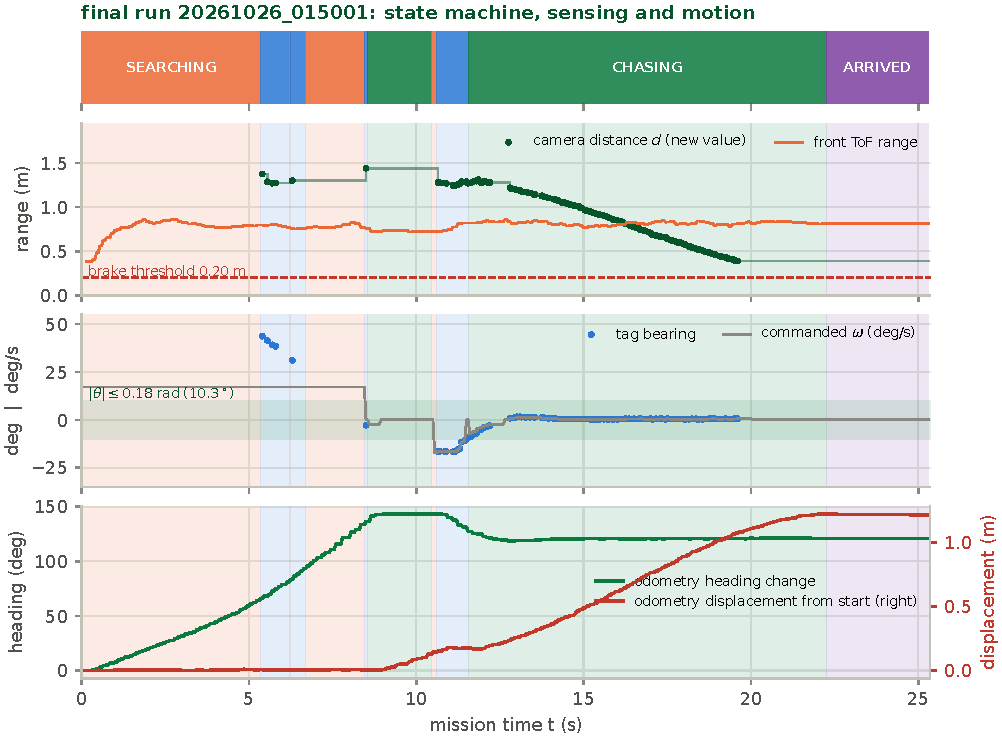
\includegraphics[width=\linewidth]{figures/p5_timeline.pdf}
\caption{Final run in detail. Camera range (new detections as dots) and ToF range; tag bearing with the
$\pm0.18$\,rad window and the commanded yaw rate; odometry heading change and displacement.}
\label{fig:timeline}
\end{figure}

\begin{itemize}
  \item \textbf{SEARCHING (0 to 5.35\,s):} counter-clockwise sweep at 0.30\,rad/s; odometry shows $65.8^\circ$ of
        rotation before T3 entered the image at its left edge ($+43.7^\circ$).
  \item \textbf{ALIGNING with flicker (5.35 to 8.55\,s):} at 1.3 to 1.4\,m the tag was at the edge of its range and of
        the image, so detections came and went and the state alternated with SEARCHING. Both states kept turning
        toward the tag (the search side follows the last bearing), so the sweep continued until T3 was centered
        ($\theta=-0.049$\,rad).
  \item \textbf{First chase (8.60 to 10.45\,s):} started from $d_0=1.440$\,m; a detection gap longer than 2.0\,s
        returned the robot to SEARCHING after 0.13\,m.
  \item \textbf{Re-alignment (10.50 to 11.55\,s):} the sweep went clockwise (last bearing negative), T3 reappeared
        at $-16.4^\circ$ ($-0.287$\,rad) and was centered in about 1\,s.
  \item \textbf{Final chase (11.60 to 22.25\,s):} $d_0=1.269$\,m, $T=10.69$\,s; from 12.8\,s about 13 new
        detections/s (gaps $\le0.2$\,s) until the tag left the image at 0.391\,m (19.60\,s); the plan carried the robot through the blind zone and
        ended at $t=T$. ARRIVED at 22.30\,s, tape standoff \textbf{20\,cm}.
\end{itemize}

\begin{figure}[H]
\centering
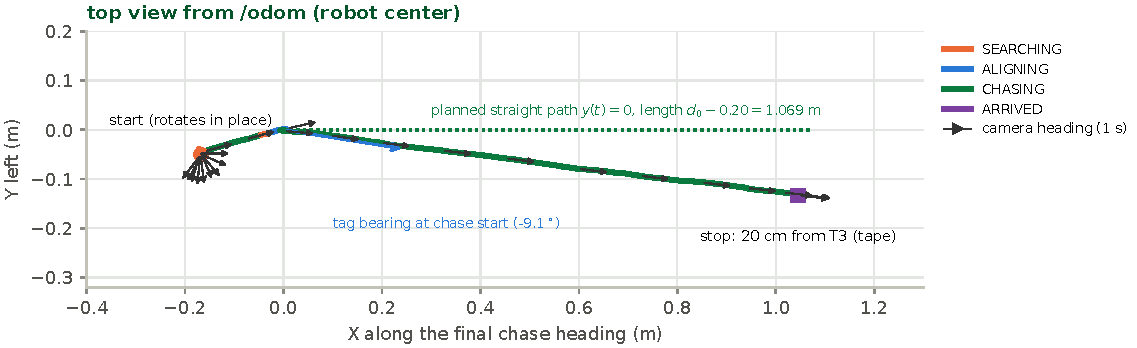
\includegraphics[width=\linewidth]{figures/p5_topview.pdf}
\caption{Path of the robot center from \code{/odom}, rotated so that the final chase starts at the origin along $+X$.
The in-place sweep appears as the cluster of heading arrows at the start; the final chase bends slightly right,
toward the tag that was at $-9.1^\circ$ when it started.}
\label{fig:topview}
\end{figure}

\isub{\faFilm}{Demonstration video}
\begin{itemize}
  \item \textbf{File:} \code{video/A2_demo_side_by_side.mp4}, 23.8\,s ($\le45$\,s), 1920$\times$480 at 30\,fps:
        \link{\videolink}{\faVideo\ demo video}.
  \item \textbf{Layout:} phone recording of the robot (left), robot camera with the T3 detection box (middle) and a top
        view of the driven path against the planned cubic $z(t)$ (right). The overlay shows mission time, state,
        $d$, $\theta$ and the command.
  \item \textbf{Content:} (a) sweep in place while T3 is hidden, (b) centering when T3 is spotted, (c) cruise and stop at
        20\,cm. Figure~\ref{fig:stills} shows one frame of each phase.
\end{itemize}

\begin{figure}[p]
\centering
\begin{subfigure}{\linewidth}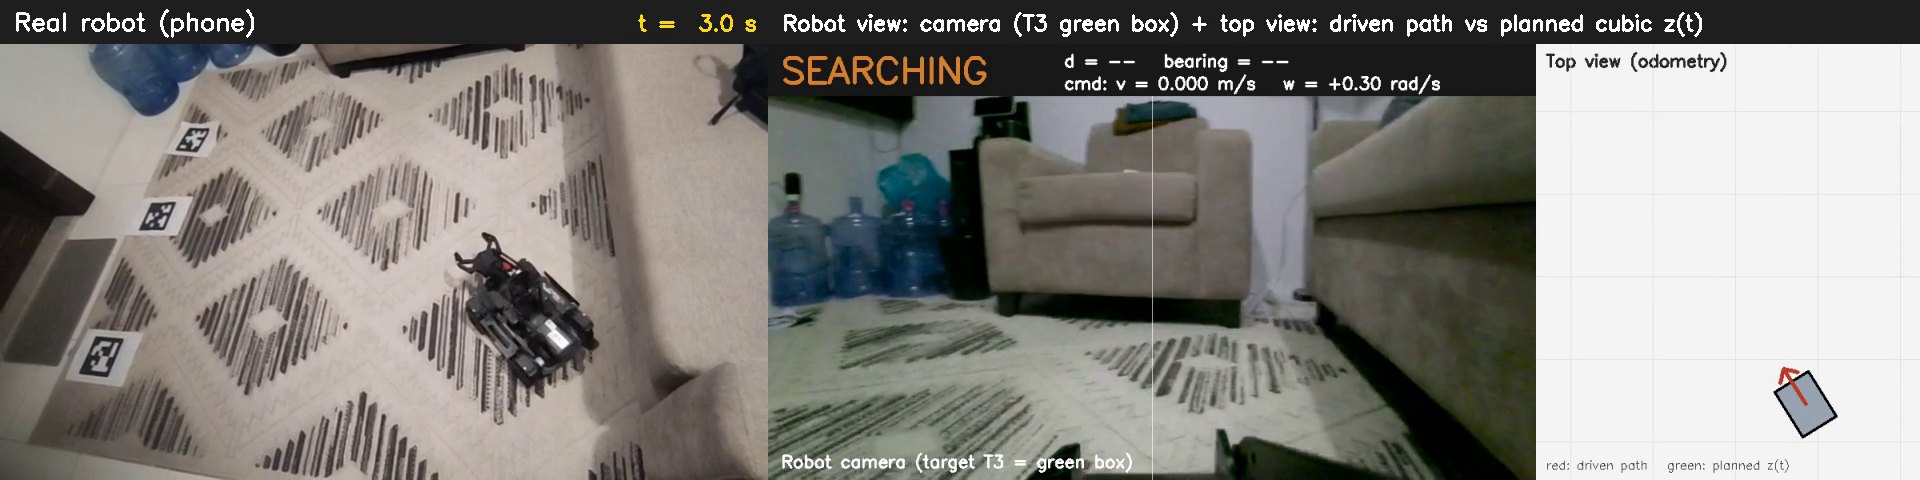
\includegraphics[width=\linewidth]{figures/still_searching.jpg}
\caption{SEARCHING, $t=3.0$\,s: sweeping counter-clockwise, T3 (left in the phone view) is outside the camera view.}\end{subfigure}\\[3pt]
\begin{subfigure}{\linewidth}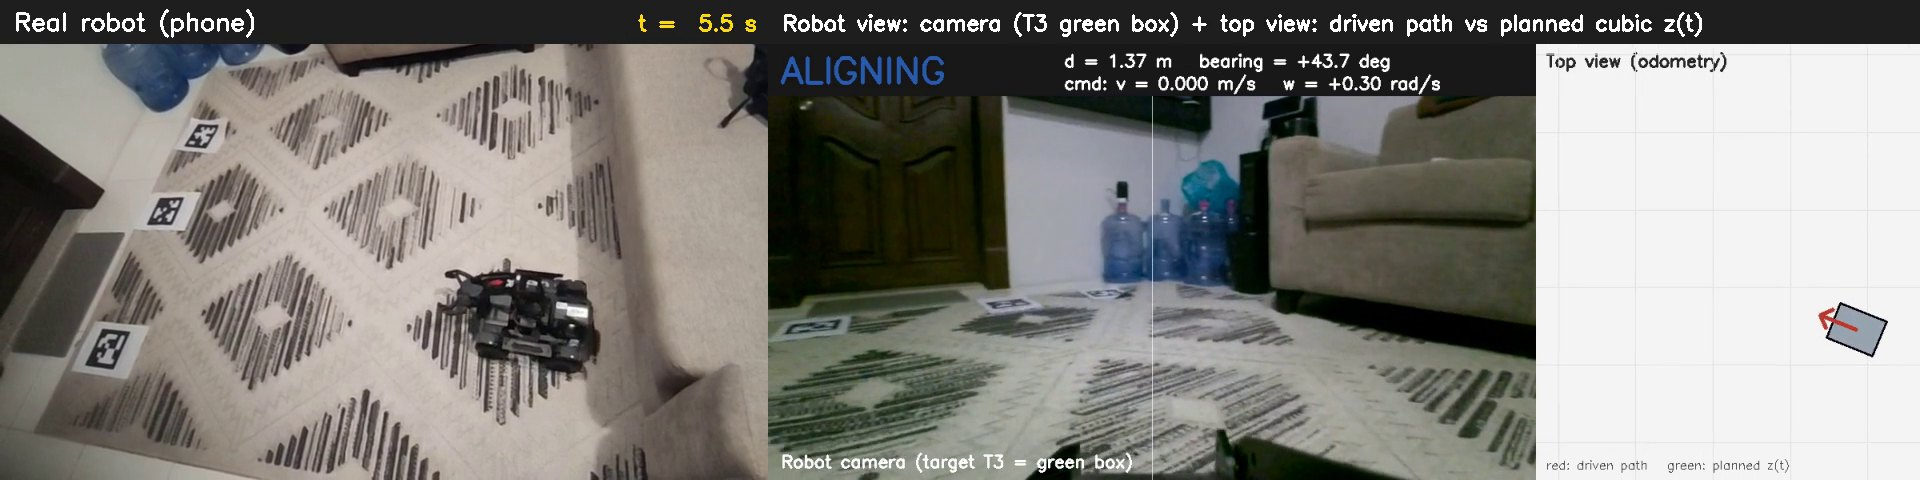
\includegraphics[width=\linewidth]{figures/still_aligning.jpg}
\caption{ALIGNING, $t=5.5$\,s: T3 just entered the camera image at $\theta=+43.7^\circ$, $d=1.37$\,m.}\end{subfigure}\\[3pt]
\begin{subfigure}{\linewidth}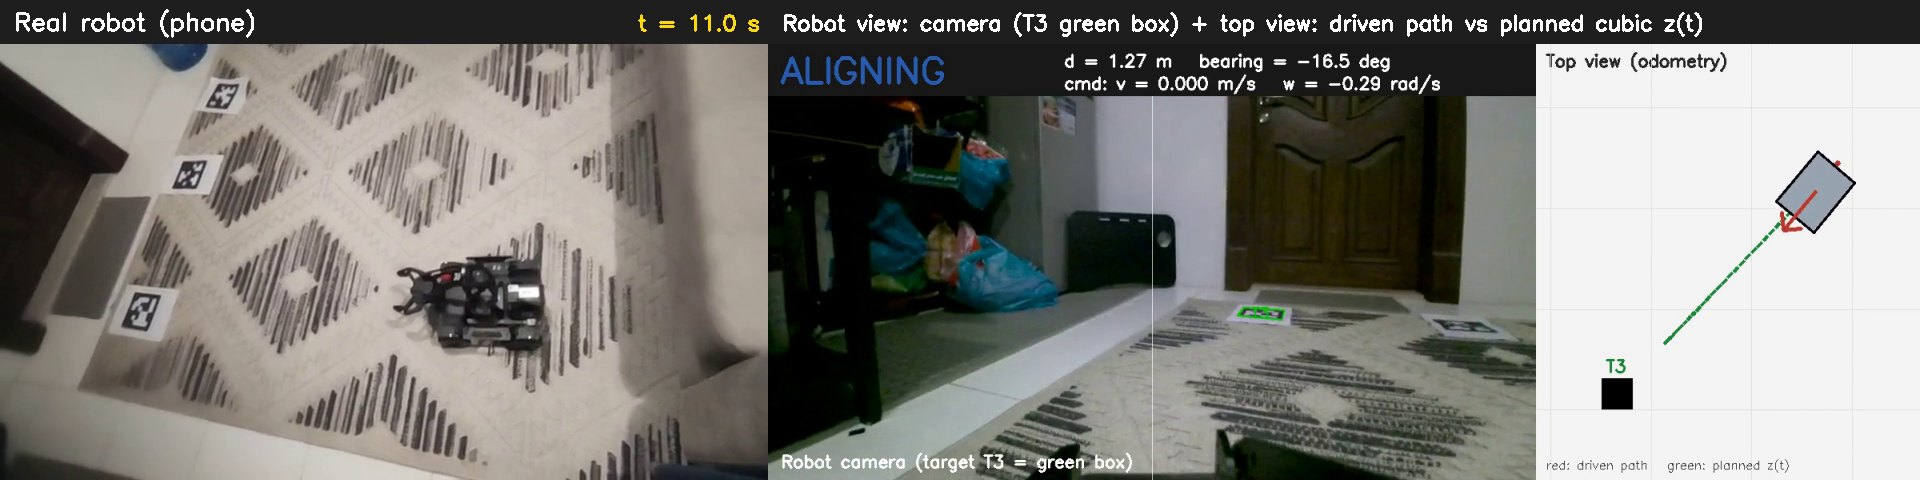
\includegraphics[width=\linewidth]{figures/still_realign.jpg}
\caption{ALIGNING again, $t=11.0$\,s: after the detection gap, T3 (green box) is centered with $\omega=-0.29$\,rad/s.}\end{subfigure}\\[3pt]
\begin{subfigure}{\linewidth}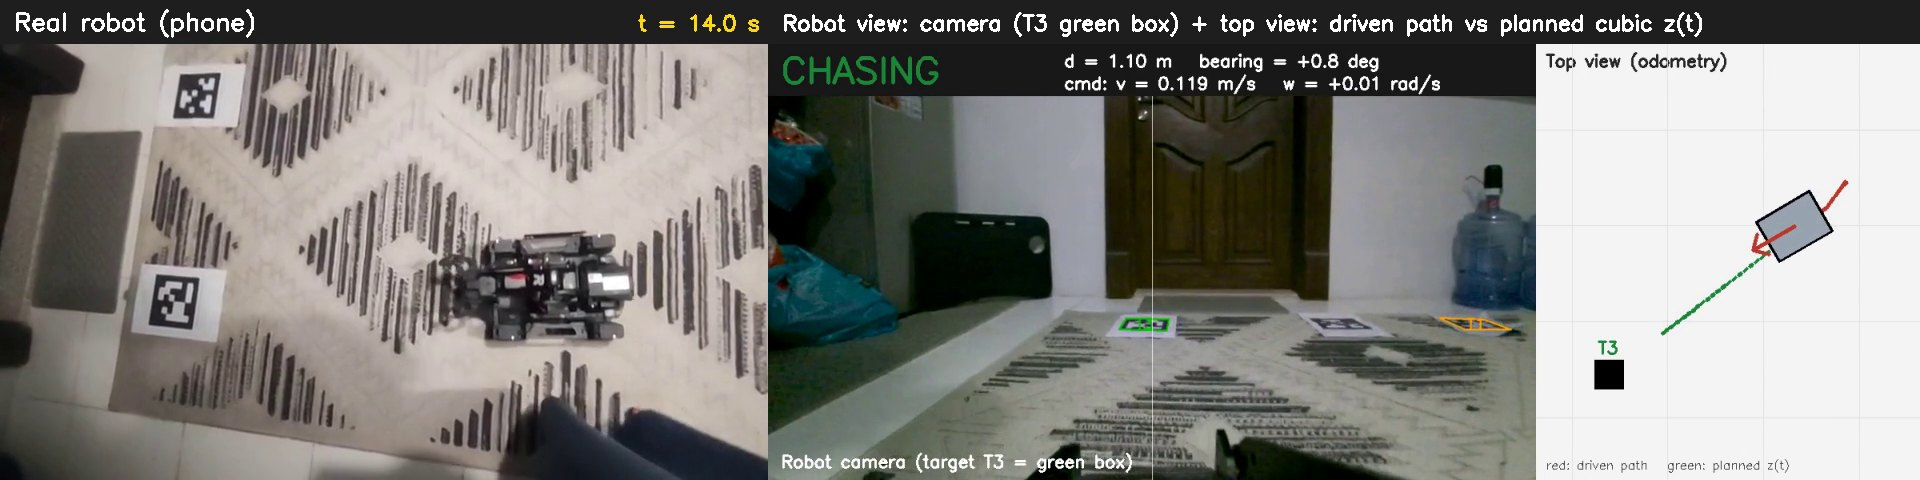
\includegraphics[width=\linewidth]{figures/still_chasing.jpg}
\caption{CHASING, $t=14.0$\,s: $d=1.10$\,m, $v=0.119$\,m/s along the cubic plan (green dots in the top view).}\end{subfigure}\\[3pt]
\begin{subfigure}{\linewidth}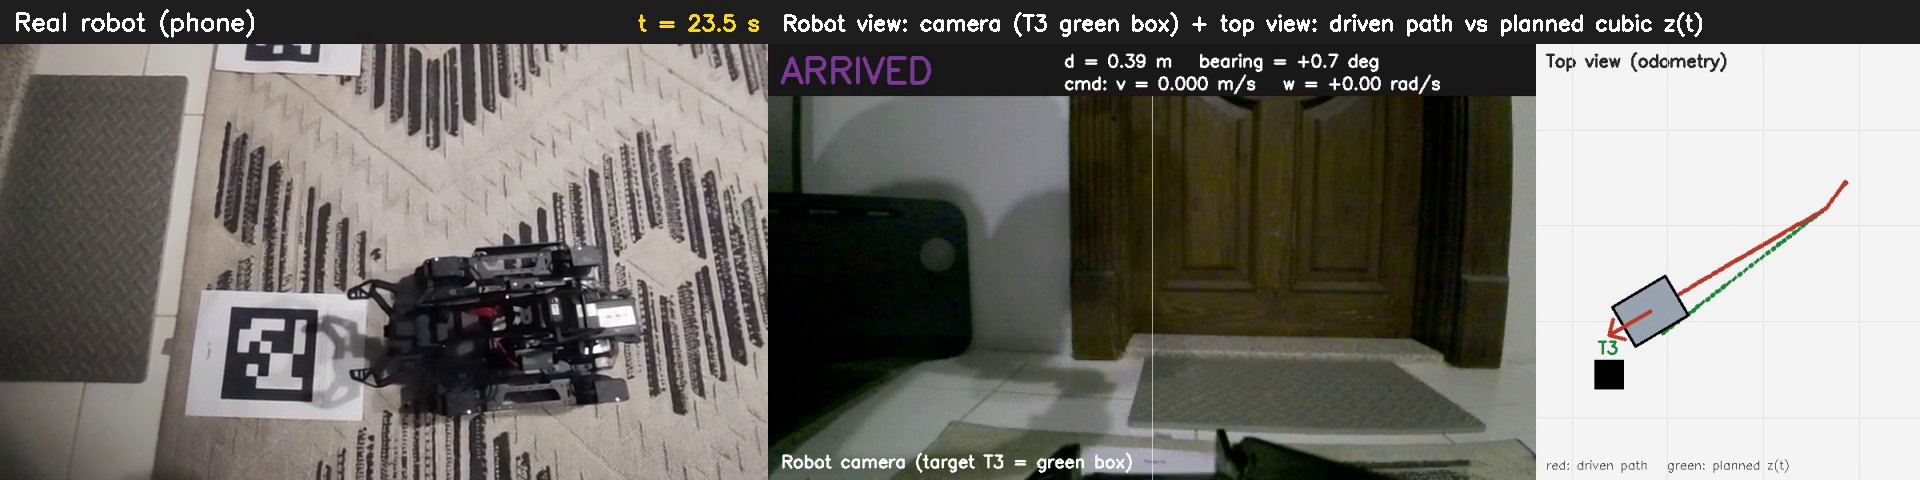
\includegraphics[width=\linewidth]{figures/still_arrived.jpg}
\caption{ARRIVED, $t=23.5$\,s: stopped 20\,cm before T3 (tape), command zero, all motor voltages 0.000\,V.}\end{subfigure}
\caption{Frames of the demonstration video (phone view, robot camera, top view).}
\label{fig:stills}
\end{figure}
